\begin{flushright} {\tiny {\color{gray} whatisafieldstone.tex}} \end{flushright}

\begin{center}
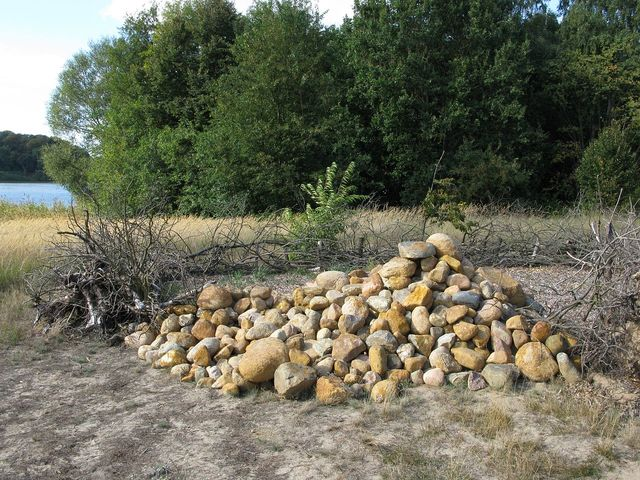
\includegraphics[width=5cm]{images/fieldstone2}\\
{\captionfont Taken from \url{https://en.wikipedia.org/wiki/Fieldstone}}
\end{center}

Simply put, it is a stone collected from the surface of fields where it 
occurs naturally. It also stands for the bad acronym: {\sl fi}nite 
{\sl el}ement {\sl d}eformation of {\sl stone}s which echoes the primary 
application of these codes: geodynamic modelling.
